% Options for packages loaded elsewhere
\PassOptionsToPackage{unicode}{hyperref}
\PassOptionsToPackage{hyphens}{url}
%
\documentclass[
]{article}
\usepackage{amsmath,amssymb}
\usepackage{lmodern}
\usepackage{ifxetex,ifluatex}
\ifnum 0\ifxetex 1\fi\ifluatex 1\fi=0 % if pdftex
  \usepackage[T1]{fontenc}
  \usepackage[utf8]{inputenc}
  \usepackage{textcomp} % provide euro and other symbols
\else % if luatex or xetex
  \usepackage{unicode-math}
  \defaultfontfeatures{Scale=MatchLowercase}
  \defaultfontfeatures[\rmfamily]{Ligatures=TeX,Scale=1}
\fi
% Use upquote if available, for straight quotes in verbatim environments
\IfFileExists{upquote.sty}{\usepackage{upquote}}{}
\IfFileExists{microtype.sty}{% use microtype if available
  \usepackage[]{microtype}
  \UseMicrotypeSet[protrusion]{basicmath} % disable protrusion for tt fonts
}{}
\makeatletter
\@ifundefined{KOMAClassName}{% if non-KOMA class
  \IfFileExists{parskip.sty}{%
    \usepackage{parskip}
  }{% else
    \setlength{\parindent}{0pt}
    \setlength{\parskip}{6pt plus 2pt minus 1pt}}
}{% if KOMA class
  \KOMAoptions{parskip=half}}
\makeatother
\usepackage{xcolor}
\IfFileExists{xurl.sty}{\usepackage{xurl}}{} % add URL line breaks if available
\IfFileExists{bookmark.sty}{\usepackage{bookmark}}{\usepackage{hyperref}}
\hypersetup{
  pdftitle={IDS 702 Team Black Project},
  pdfauthor={Emma Wang, Pragya Raghuvanshi, Lorna Aine, Eric Rios Soderman},
  hidelinks,
  pdfcreator={LaTeX via pandoc}}
\urlstyle{same} % disable monospaced font for URLs
\usepackage[margin=1in]{geometry}
\usepackage{color}
\usepackage{fancyvrb}
\newcommand{\VerbBar}{|}
\newcommand{\VERB}{\Verb[commandchars=\\\{\}]}
\DefineVerbatimEnvironment{Highlighting}{Verbatim}{commandchars=\\\{\}}
% Add ',fontsize=\small' for more characters per line
\usepackage{framed}
\definecolor{shadecolor}{RGB}{248,248,248}
\newenvironment{Shaded}{\begin{snugshade}}{\end{snugshade}}
\newcommand{\AlertTok}[1]{\textcolor[rgb]{0.94,0.16,0.16}{#1}}
\newcommand{\AnnotationTok}[1]{\textcolor[rgb]{0.56,0.35,0.01}{\textbf{\textit{#1}}}}
\newcommand{\AttributeTok}[1]{\textcolor[rgb]{0.77,0.63,0.00}{#1}}
\newcommand{\BaseNTok}[1]{\textcolor[rgb]{0.00,0.00,0.81}{#1}}
\newcommand{\BuiltInTok}[1]{#1}
\newcommand{\CharTok}[1]{\textcolor[rgb]{0.31,0.60,0.02}{#1}}
\newcommand{\CommentTok}[1]{\textcolor[rgb]{0.56,0.35,0.01}{\textit{#1}}}
\newcommand{\CommentVarTok}[1]{\textcolor[rgb]{0.56,0.35,0.01}{\textbf{\textit{#1}}}}
\newcommand{\ConstantTok}[1]{\textcolor[rgb]{0.00,0.00,0.00}{#1}}
\newcommand{\ControlFlowTok}[1]{\textcolor[rgb]{0.13,0.29,0.53}{\textbf{#1}}}
\newcommand{\DataTypeTok}[1]{\textcolor[rgb]{0.13,0.29,0.53}{#1}}
\newcommand{\DecValTok}[1]{\textcolor[rgb]{0.00,0.00,0.81}{#1}}
\newcommand{\DocumentationTok}[1]{\textcolor[rgb]{0.56,0.35,0.01}{\textbf{\textit{#1}}}}
\newcommand{\ErrorTok}[1]{\textcolor[rgb]{0.64,0.00,0.00}{\textbf{#1}}}
\newcommand{\ExtensionTok}[1]{#1}
\newcommand{\FloatTok}[1]{\textcolor[rgb]{0.00,0.00,0.81}{#1}}
\newcommand{\FunctionTok}[1]{\textcolor[rgb]{0.00,0.00,0.00}{#1}}
\newcommand{\ImportTok}[1]{#1}
\newcommand{\InformationTok}[1]{\textcolor[rgb]{0.56,0.35,0.01}{\textbf{\textit{#1}}}}
\newcommand{\KeywordTok}[1]{\textcolor[rgb]{0.13,0.29,0.53}{\textbf{#1}}}
\newcommand{\NormalTok}[1]{#1}
\newcommand{\OperatorTok}[1]{\textcolor[rgb]{0.81,0.36,0.00}{\textbf{#1}}}
\newcommand{\OtherTok}[1]{\textcolor[rgb]{0.56,0.35,0.01}{#1}}
\newcommand{\PreprocessorTok}[1]{\textcolor[rgb]{0.56,0.35,0.01}{\textit{#1}}}
\newcommand{\RegionMarkerTok}[1]{#1}
\newcommand{\SpecialCharTok}[1]{\textcolor[rgb]{0.00,0.00,0.00}{#1}}
\newcommand{\SpecialStringTok}[1]{\textcolor[rgb]{0.31,0.60,0.02}{#1}}
\newcommand{\StringTok}[1]{\textcolor[rgb]{0.31,0.60,0.02}{#1}}
\newcommand{\VariableTok}[1]{\textcolor[rgb]{0.00,0.00,0.00}{#1}}
\newcommand{\VerbatimStringTok}[1]{\textcolor[rgb]{0.31,0.60,0.02}{#1}}
\newcommand{\WarningTok}[1]{\textcolor[rgb]{0.56,0.35,0.01}{\textbf{\textit{#1}}}}
\usepackage{longtable,booktabs,array}
\usepackage{calc} % for calculating minipage widths
% Correct order of tables after \paragraph or \subparagraph
\usepackage{etoolbox}
\makeatletter
\patchcmd\longtable{\par}{\if@noskipsec\mbox{}\fi\par}{}{}
\makeatother
% Allow footnotes in longtable head/foot
\IfFileExists{footnotehyper.sty}{\usepackage{footnotehyper}}{\usepackage{footnote}}
\makesavenoteenv{longtable}
\usepackage{graphicx}
\makeatletter
\def\maxwidth{\ifdim\Gin@nat@width>\linewidth\linewidth\else\Gin@nat@width\fi}
\def\maxheight{\ifdim\Gin@nat@height>\textheight\textheight\else\Gin@nat@height\fi}
\makeatother
% Scale images if necessary, so that they will not overflow the page
% margins by default, and it is still possible to overwrite the defaults
% using explicit options in \includegraphics[width, height, ...]{}
\setkeys{Gin}{width=\maxwidth,height=\maxheight,keepaspectratio}
% Set default figure placement to htbp
\makeatletter
\def\fps@figure{htbp}
\makeatother
\setlength{\emergencystretch}{3em} % prevent overfull lines
\providecommand{\tightlist}{%
  \setlength{\itemsep}{0pt}\setlength{\parskip}{0pt}}
\setcounter{secnumdepth}{-\maxdimen} % remove section numbering
\usepackage{booktabs}
\usepackage{longtable}
\usepackage{array}
\usepackage{multirow}
\usepackage{wrapfig}
\usepackage{float}
\usepackage{colortbl}
\usepackage{pdflscape}
\usepackage{tabu}
\usepackage{threeparttable}
\usepackage{threeparttablex}
\usepackage[normalem]{ulem}
\usepackage{makecell}
\usepackage{xcolor}
\ifluatex
  \usepackage{selnolig}  % disable illegal ligatures
\fi

\title{IDS 702 Team Black Project}
\author{Emma Wang, Pragya Raghuvanshi, Lorna Aine, Eric Rios Soderman}
\date{2022-10-21}

\begin{document}
\maketitle

\hypertarget{exploring-popularity-and-explicity-of-2010s-music-through-musicality.}{%
\section{EXPLORING POPULARITY AND EXPLICITY OF 2010s MUSIC THROUGH
MUSICALITY.}\label{exploring-popularity-and-explicity-of-2010s-music-through-musicality.}}

\hypertarget{i.-data-overview}{%
\subsection{I. Data Overview}\label{i.-data-overview}}

The data set used in this research is a subset of a larger
\href{https://www.kaggle.com/datasets/yamaerenay/spotify-dataset-19212020-600k-tracks}{spotify
dataset} that contained 586672 tracks. Our final subset of the data set
of interest to our research problems contains 104767of observations/
tracks and 23 of variables for songs between 2010 and 2019. Our focus in
this research is to infer which features of music are best associated to
the popularity of songs and to predict if a song will be explicit or not
based on these features.

After examining this data set, we decided on investigating two key
problems of interest. One was gauging song popularity, and the other was
predicting a song's explicitness. For the former, we were profoundly
intrigued by what song features or musical attributes effectively gauged
and predicted a song's popularity. For the latter, we focused on
validating what features of a song best predicted if a song was likely
to be explicit or non-explicit. Explicitness refers to the use of slurs
and inappropriate words in a song. For both, we choose the variables
based on prior domain knowledge.

Our Research Questions:

-What are the musical attributes that gauged the popularity of songs in
the 2010s? \emph{Dependent Variable (continuous) = popularity}
\emph{Independent Variables = acousticness, danceability, energy,
instrumentation, tempo, loudness, and speechiness}

-To what extent can the musicality of a song predict whether a song will
be explicit or non-explicit? \emph{Dependent Variable (categorical) =
Explicitness} \emph{Independent Variables = danceability, energy,
speechiness, and tempo}

\hypertarget{ii.primary-relationship-of-interest}{%
\subsection{II.Primary relationship of
interest}\label{ii.primary-relationship-of-interest}}

To better understand the various variables that gauge the musicality of
a song, we will include the definitions of our main variables of
interest, which were sourced from Spotify's API documentation.

\hypertarget{definitions-of-variables-of-interest}{%
\subsubsection{Definitions of variables of
interest}\label{definitions-of-variables-of-interest}}

-\textbf{Popularity} is calculated by an algorithm that is based on how
many times a track has been played and how recent those plays were. This
is the response variable of interest for research question 1 (Spotify,
2022).

-\textbf{Explicitness} is whether a song contains inappropriate words
such as curse words and sexually explicit words that are unacceptable to
play in some public settings. 1 is the value identifying a song as
explicit, while 0 implies that a song is non-explicit. This is the
dependent variable for the second research question (Spotify, 2022).

-**Acousticness* is a confidence measure from 0.0 to 1.0 of how much of
the track is composed with acoustic instruments. 1.0 represents high
confidence the track is acoustic (Spotify, 2022).

-\textbf{Danceability} is a rating of a track's suitability for dancing.
This metric is based on a combination of musical elements including
tempo, rhythm stability, beat strength, and overall regularity. A value
of 0.0 is least danceable and 1.0 is most danceable (Spotify, 2022).

-**Energy* is a perceptual measure of intensity and activity. Energetic
tracks typically feel fast, loud, and noisy (Spotify, 2022).

-\textbf{Instrumentation} pertains to whether a track contains no
vocals. ``Ooh'' and ``aah'' sounds are treated as instrumentals in this
context, while Rap or spoken word tracks are considered ``vocal''. As
the instrumentalness value approaches 1.0, there is a greater likelihood
that the track contains no vocal content. In addition, values above 0.5
are intended to represent instrumental tracks, but confidence is higher
as the value approaches 1.0 (Spotify, 2022).

-\textbf{Tempo} refers to the overall estimated tempo of a track in
beats per minute (BPM). In musical terminology, tempo is the speed or
pace of a given piece, which derives directly from the average beat
duration (Spotify, 2022).

-\textbf{Loudness} measures the overall loudness of a track in decibels
(dB). Loudness values are averaged across the entire track and are
useful for comparing relative loudness of tracks. Loudness is the
quality of a sound that is the primary psychological association of
physical strength (amplitude). Lastly, the values typically range
between -60 and 0 db (Spotify, 2022).

-\textbf{Speechiness} detects the presence of spoken words in a track.
The more exclusively speech-like the recording (e.g.~talk show, audio
book, poetry), the closer to 1.0 the attribute value. Values above 0.66
describe tracks that are probably made entirely of spoken words. Values
between 0.33 and 0.66 describe tracks that may contain both music and
speech, either in sections or layered, including such cases as rap
music. Values below 0.33 most likely represent music and other
non-speech-like tracks (Spotify, 2022).

\hypertarget{justification-for-variable-selection}{%
\subsubsection{Justification for Variable
Selection}\label{justification-for-variable-selection}}

First and foremost, we chose the variables for our research questions
based on prior, domain knowledge of musical terminology. For the first
research question, which concerns the features that popularized songs
during the 2010s, a series of aforementioned predictors were chosen.
What will follow is the justification for this ``a priori'' selection
for both research questions.

The reasoning for choosing these specific predictors (acousticness,
danceability, energy, instrumentation, tempo, loudness, and speechiness)
to predict song popularity is the weight of their importance. Popular
songs, whether they are an emotional ballad or a dance track, all have
certain features to keep the listeners engaged and interested to repeat
listening to these tracks (Leviatan, 2017). The tempo, energy and
loudness indicate the pacing and sonic impact and pleasantness of the
track. The speechiness, danceability and instrumentation (which also
includes acoustic choices or ``acousticness'') dictate melody choices,
chord progressions, instrument choices, wordings, vocal lines and more
types sonic layers. However, this last point is very nuanced because it
pertains to the genre choice of the producers. There are very popular
songs with high instrumentation, no words and low danceability, such as
songs from classical music. On the other hand, Pop and Rock songs vary
their levels of instrumentation and acousticness and speechiness to
deliver the best possible songs. Lastly, if the song is aimed towards a
festive audience, such as a club song, then prioritizing danceability
governs the levels of instrumentation and speechiness and lack of
acousticness, and this prioritization varies by genre (Androids, 2017).
In conclusion, the interplay of these factors influence the popularity
of songs by helping them become easily memorable and enticing.

As for the second research question, the explicitness of tracks is
strongly swayed by other factors. A very logical approach to predicting
explicitness was first looking at the high levels of speechiness in
songs. For example, rap songs rank high in this metric because the
verses are composed of a spoken word format over a series of 8 or 16
bars, and each bar is a rap line (Edwords), while singing doesn't have
to adhere to the ``1 bar = 1 line'' rule; thus, speechiness became the
metric of most importance. In addition, songs in this genre tend to
include explicit content, often sexual, in the lyrics (Tayag, 2017).
Second to this metric, the other predictors of danceability, energy and
tempo were considered as helpful in predicing explicitness. The energy
and danceability of the song collude with speechiness to infer if a
track could have explicit language. For example, a song with low energy
and low danceability may or may not be less likely to have explicit
language than a song with high energy and danceability, holding the
speechiness level constant, and this is a relationship we wish to
investigate as well. As for tempo, music genres that are known to
include explicit language follow specific tempos. For instance, Trap
songs usually have a tempo of 140 bpm (Burchell, 2019).

To fully understand the data with which we are working, we will explore
the basic statistics of the variables of interest.

\begin{tabular}[t]{llll}
\toprule
  & Non-Explicit & Explicit & total\\
\midrule
 & (N=92440) & (N=12327) & (N=104767)\\
\addlinespace[0.3em]
\multicolumn{4}{l}{\textbf{acousticness}}\\
\hspace{1em}Mean (SD) & 0.295 (0.300) & 0.227 (0.224) & 0.287 (0.293)\\
\hspace{1em}Median [Min, Max] & 0.181 [0, 0.996] & 0.151 [0.00000115, 0.993] & 0.176 [0, 0.996]\\
\addlinespace[0.3em]
\multicolumn{4}{l}{\textbf{danceability}}\\
\hspace{1em}Mean (SD) & 0.599 (0.154) & 0.687 (0.147) & 0.609 (0.156)\\
\hspace{1em}Median [Min, Max] & 0.609 [0.0532, 0.988] & 0.708 [0.0620, 0.986] & 0.620 [0.0532, 0.988]\\
\addlinespace[0.3em]
\multicolumn{4}{l}{\textbf{energy}}\\
\hspace{1em}Mean (SD) & 0.657 (0.224) & 0.680 (0.162) & 0.660 (0.217)\\
\hspace{1em}Median [Min, Max] & 0.692 [0.0000203, 1.00] & 0.685 [0.0000202, 1.00] & 0.691 [0.0000202, 1.00]\\
\addlinespace[0.3em]
\multicolumn{4}{l}{\textbf{instrumentalness}}\\
\hspace{1em}Mean (SD) & 0.0975 (0.254) & 0.0212 (0.110) & 0.0885 (0.243)\\
\hspace{1em}Median [Min, Max] & 0.00000368 [0, 1.00] & 0 [0, 0.989] & 0.00000251 [0, 1.00]\\
\addlinespace[0.3em]
\multicolumn{4}{l}{\textbf{tempo}}\\
\hspace{1em}Mean (SD) & 123 (28.2) & 120 (29.4) & 122 (28.3)\\
\hspace{1em}Median [Min, Max] & 124 [31.3, 230] & 120 [46.7, 220] & 124 [31.3, 230]\\
\addlinespace[0.3em]
\multicolumn{4}{l}{\textbf{loudness}}\\
\hspace{1em}Mean (SD) & -7.32 (3.90) & -6.71 (2.56) & -7.25 (3.77)\\
\hspace{1em}Median [Min, Max] & -6.52 [-54.8, 1.93] & -6.40 [-29.0, 1.26] & -6.50 [-54.8, 1.93]\\
\addlinespace[0.3em]
\multicolumn{4}{l}{\textbf{speechiness}}\\
\hspace{1em}Mean (SD) & 0.0752 (0.0754) & 0.188 (0.130) & 0.0885 (0.0912)\\
\hspace{1em}Median [Min, Max] & 0.0461 [0.0220, 0.658] & 0.159 [0.0229, 0.658] & 0.0497 [0.0220, 0.658]\\
\addlinespace[0.3em]
\multicolumn{4}{l}{\textbf{popularity}}\\
\hspace{1em}Mean (SD) & 38.1 (19.5) & 47.7 (17.4) & 39.2 (19.5)\\
\hspace{1em}Median [Min, Max] & 42.0 [0, 92.0] & 50.0 [0, 94.0] & 42.0 [0, 94.0]\\
\bottomrule
\end{tabular}

From the table below, we can observe the mean, median, standard
deviation, minimum and maximum values of variables separately for
explicit and non explicit categories. While mean values of acousticness,
instrumentalness, tempo are higher for non explicit songs, values for
energy, danceability, loudness and speechiness are higher for explicit
songs. In addition, we can also infer that popularity of explicit songs
is minutely higher than non explicit songs. As for standard deviation,
high values for tempo and popularity indicate that the data points are
spread out in relation to the mean value, whereas low values for
danceability, energy, speechiness indicate that the data points are
clustered around the mean. Lastly, nearly equal values of median and
mean for danceability, energy and tempo indicate that the data points
are more or less evenly distributed.

One way to ascertain the weight of association amongst predictors is to
create a correlation matrix, where each variable's relationship to one
another is quantified.

\begin{Shaded}
\begin{Highlighting}[]
\NormalTok{RQ1\_relation }\OtherTok{\textless{}{-}} \FunctionTok{c}\NormalTok{(}\StringTok{"popularity"}\NormalTok{, }\StringTok{"acousticness"}\NormalTok{, }\StringTok{"danceability"}\NormalTok{, }\StringTok{"energy"}\NormalTok{, }\StringTok{"instrumentalness"}\NormalTok{, }\StringTok{"tempo"}\NormalTok{, }\StringTok{"loudness"}\NormalTok{, }\StringTok{"speechiness"}\NormalTok{)}
\NormalTok{df1 }\OtherTok{=}\NormalTok{ subset[RQ1\_relation]}
\NormalTok{RQ2\_relation }\OtherTok{\textless{}{-}} \FunctionTok{c}\NormalTok{(}\StringTok{"explicit\_fac"}\NormalTok{, }\StringTok{"danceability"}\NormalTok{, }\StringTok{"energy"}\NormalTok{, }\StringTok{"speechiness"}\NormalTok{,}\StringTok{"tempo"}\NormalTok{)}
\NormalTok{df2 }\OtherTok{=}\NormalTok{ subset[RQ2\_relation]}
\NormalTok{cordf1 }\OtherTok{=} \FunctionTok{cor}\NormalTok{(df1)}
\FunctionTok{corrplot}\NormalTok{(cordf1, }\AttributeTok{method =} \StringTok{\textquotesingle{}color\textquotesingle{}}\NormalTok{, }\AttributeTok{order =} \StringTok{\textquotesingle{}alphabet\textquotesingle{}}\NormalTok{)}
\end{Highlighting}
\end{Shaded}

\includegraphics{IDS-702-Team-Black-Project_files/figure-latex/unnamed-chunk-4-1.pdf}

Based on the results, except one case, the variables are weakly
correlated with each other. On the other hand, the one exception was
acousticness and energy, which had a fairly strong correlation that we
will consider cautiously when we approach the modeling phase.

\hypertarget{analysis-of-variables}{%
\subsubsection{Analysis of variables}\label{analysis-of-variables}}

To better understand the data set, the popularity variable was binned
into 5 groups ranging from least popular to more popular across group 1
to group 5.

\begin{longtable}[]{@{}cc@{}}
\caption{Popularity Grouping}\tabularnewline
\toprule
Popularity\_group & Criteria \\
\midrule
\endfirsthead
\toprule
Popularity\_group & Criteria \\
\midrule
\endhead
Popularity group 1 & popularity \textless= 20 \\
Popularity group 2 & popularity \textless= 40 \\
Popularity group 3 & popularity \textless= 60 \\
Popularity group 4 & popularity \textless= 80 \\
Popularity group 4 & popularity \textless= 100 \\
\bottomrule
\end{longtable}

\includegraphics[width=0.5\linewidth]{IDS-702-Team-Black-Project_files/figure-latex/unnamed-chunk-7-1}
\includegraphics[width=0.5\linewidth]{IDS-702-Team-Black-Project_files/figure-latex/unnamed-chunk-7-2}

In Figure 1, we observe that more popular songs have a higher average
danceability than less popular songs. In Figure 2, we observe that, as
songs become more popular, the energy remains evenly distributed, but
the instrumentalness is reduced with the exception of a few outliers,
although the relationship between the two variables becomes
insignificant.

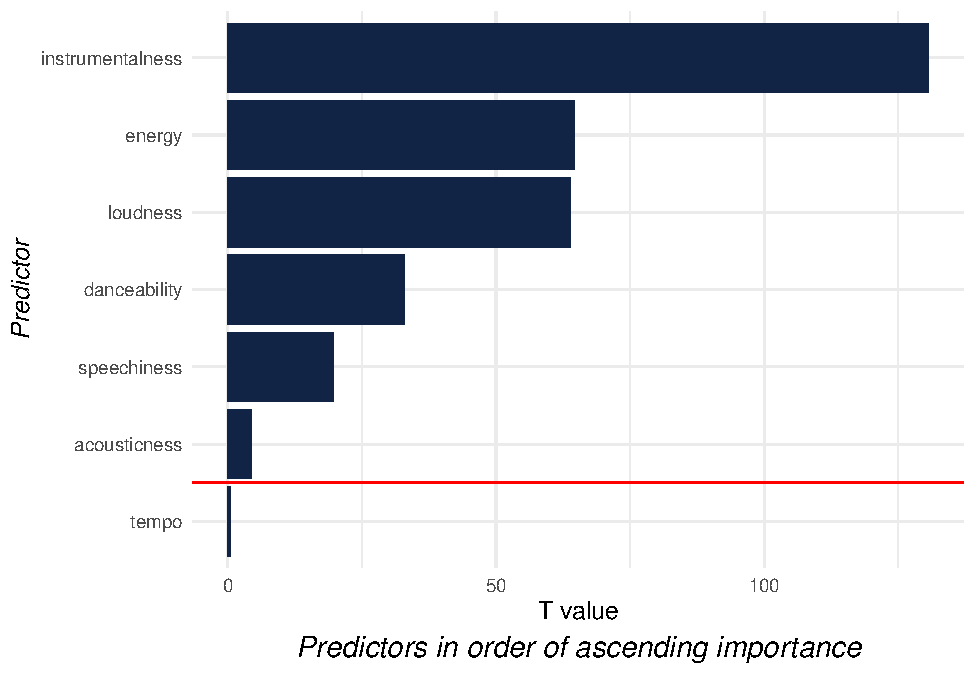
\includegraphics[width=0.5\linewidth]{IDS-702-Team-Black-Project_files/figure-latex/unnamed-chunk-8-1}
\includegraphics[width=0.5\linewidth]{IDS-702-Team-Black-Project_files/figure-latex/unnamed-chunk-8-2}

For Figure 3, the relationship between tempo and loudness reveals a very
specific recipe for the most popular, chart topping songs. This group's
tempo lies between 50-200 BPM (beats per minute) and -20 to 0 decibles.
Meanwhile, other groups' tempo and loudness profiles remain spread out
across the axes of tempo and loudness, unrestricted to a specific
quadrant of values. Similarly, for Figure 4, although the speechiness
values remain evenly distributed, the most popular songs exhibit a
massive reduction in values for instrumentation, while the less popular
songs retain a higher spread for instrumentation values. From the above
observations, if a song is massively popular (Pop Group 5), the
instrumentalness will ultimately be less signficant.

Overall, the insights show that there seems to be an assortment of
musical attributes that define an extremely popular song, yet they seem
to be less pronounced for the less popular groups of songs. In other
words, the most popular song profiles demonstrate an absence of
instrumentalness and a specific range of specific tempo and loudness
values.

EDA Q2: Fig 5 : explicit content in music has risen over the years Fig
6: the energy in explicit songs is centered around the mean(calc) while
non explicit songs are skewed to the higher energy(calc)

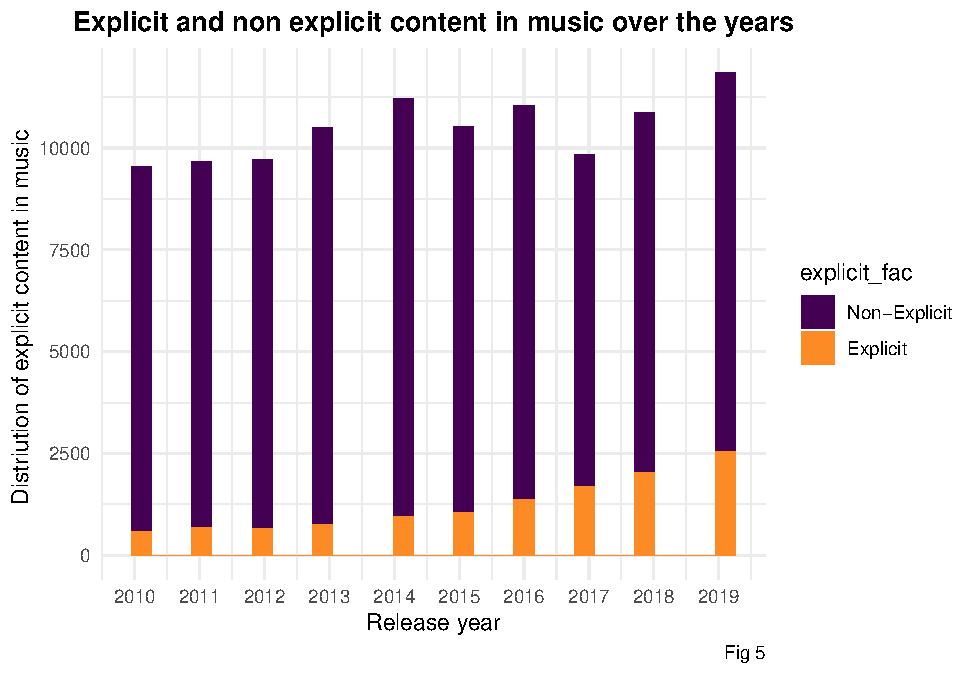
\includegraphics[width=0.5\linewidth]{IDS-702-Team-Black-Project_files/figure-latex/figures-side-1}
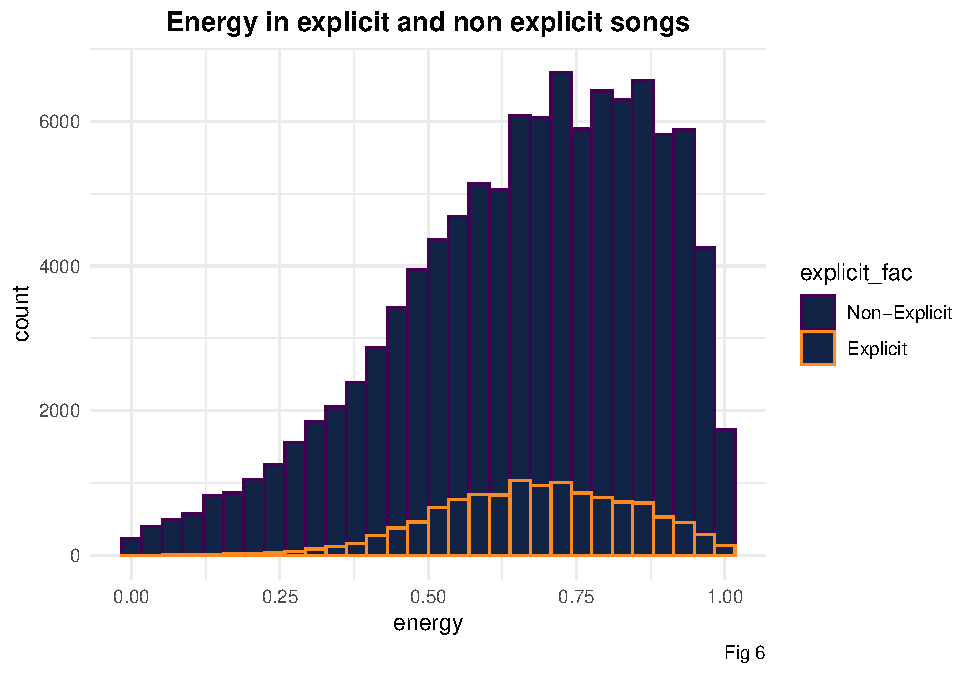
\includegraphics[width=0.5\linewidth]{IDS-702-Team-Black-Project_files/figure-latex/figures-side-2}
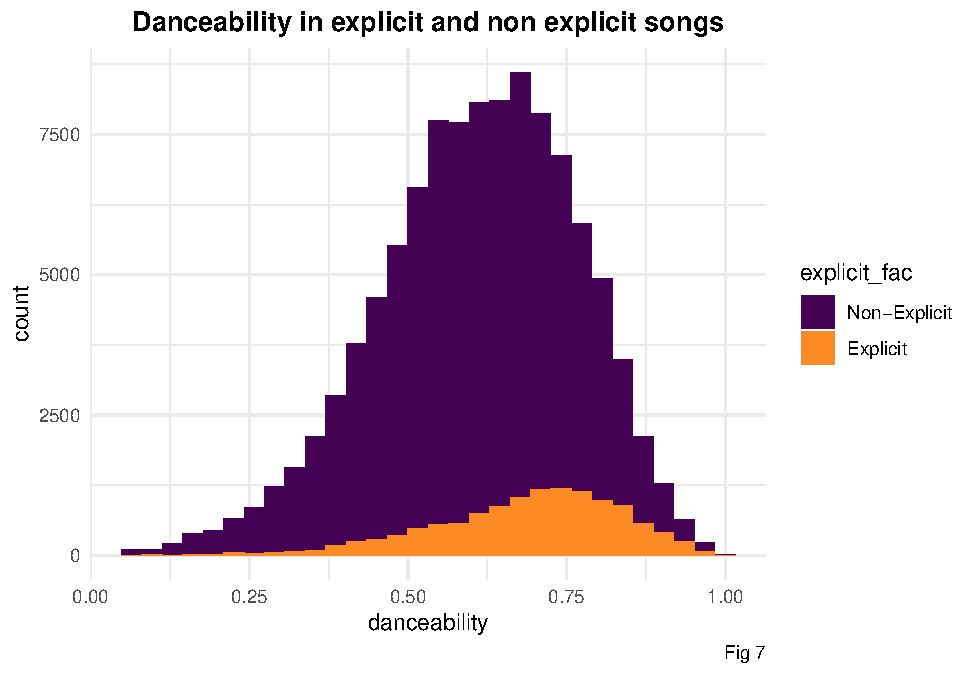
\includegraphics[width=0.5\linewidth]{IDS-702-Team-Black-Project_files/figure-latex/figures-side-3}
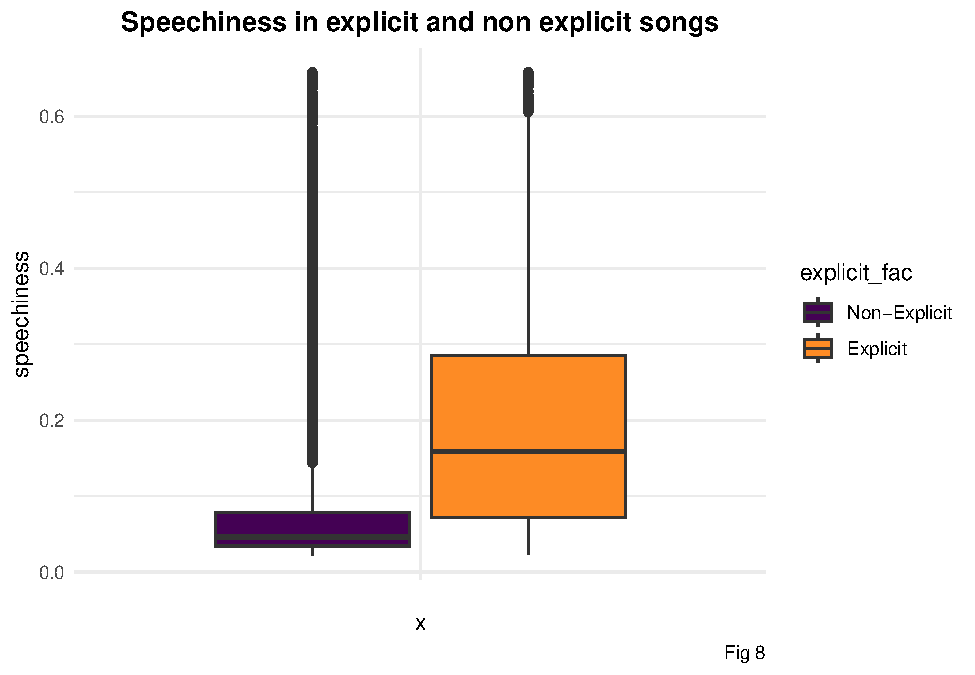
\includegraphics[width=0.5\linewidth]{IDS-702-Team-Black-Project_files/figure-latex/figures-side-4}
Fig 7: the danceability songs is centered around the mean(calc) Fig 8:
The average speechiness in explicit songs is way less in explicit songs.
In conclusion, the chosen variables would give us a great classification
of explicit and non explicit songs moving forward.

\hypertarget{iii.other-characteristics}{%
\subsection{III.Other characteristics}\label{iii.other-characteristics}}

Briefly describe other variables in the data. If there are many, do not
list them all. Rather, describe the types of variables that are present
(e.g., ``demographic information'')

A few variables such as key and time signature are part of this dataset,
although they were not chosen as the predictors. Most of the remaining
variables in this dataset pertain to the artist name, the song title,
the modalities and key of a song, the duration and the release dates.
Nonetheless, some variables were still very rich in information in terms
of prediction. To illustrate, one could predict the scale of a song
based on the popularity in addition to other predictors.

Some were not chosen because they were differently coded, such as time
signature, which has an extremely limited set of plausible values (lacks
signatures like 6/8). In contrast, some offered little or irrelevant
information. Liveness is one such case. It parametrizes a song's
performance as a live or studio quality recording, and, given that the
songs that play on the radio tend to be studio songs, we opted to not
use this variable as a predictor.

\hypertarget{iv.-potential-challenges}{%
\subsection{IV. Potential Challenges}\label{iv.-potential-challenges}}

Describe aspects of the data that may present challenges in the modeling
stage. For example, might certain categorical variables need to be
collapsed? Is there a lot of missingness? Could the size of the dataset
present model selection challenges?

Eric's findings from cleaning : Yes, there is a bit of missingness. Some
dates have years, but not months and days recorded. This meant that we
had to manually fix them or give them arbitrary values. Some artist
names are missing, which is notable but currently not obstructive. We
also do not know if some of the tempos of the higher songs were
incorrectly recorded.

Modifications based on the research questions:

\begin{enumerate}
\def\labelenumi{\arabic{enumi}.}
\item
  Our research question pertains to the songs of the 2010s decade.
  Hence, post subsetting the original dataset to our research interest,
  the dataset contains 104767 rows and 23 columns.
\item
  Bad tempo data in the subset for around 148 tracks have been dropped.
  The column names depicting are variables of interest and the rows
  depicting the number of observations.
\item
  For our first research question we have popularity as dependent
  variable which is continuous variable. Our second research questions
  predicts Explicitness(dependent variable) on basis of predictor
  variables. Explicit here is a categorical variable and hence, we will
  factor it into non explicit, and explicit.
\item
  Character was the data type for the dates column. Since the year was
  our interest, it was extracted into a new column variable as an
  integer type.
\item
  Artist names needed the brackets removed. It was cleaned for future
  use, if looking into artist's sonic profiles was our interest.
\item
  The duration variable, which was recorded in milliseconds, was
  converted to minutes to facilitate easy interpretation.
\item
  The explicitness variable needed to be factored.
\item
  For speechiness, values above 0.66 are categorized as speech tracks
  like podcasts and poetries. Hence, they have been dropped.
\item
  The tempo variable had values of 0, which is impossible for musical
  tracks. In addition, we found that tracks with these 0 values were
  often recordings of white noise, rain sounds, pink noise, intermission
  songs, and true songs with no tempo data available. These values had
  to be removed.
\end{enumerate}

\hypertarget{v.-bibliography-citations}{%
\subsection{V. Bibliography
(Citations)}\label{v.-bibliography-citations}}

Androids (2017, October 13). An Idiot's Guide to EDM Genres. Retrieved
October 20, 2022, from
\url{https://www.complex.com/music/an-idiots-guide-to-edm-genres/}

Burchell, C. (2019, May 27). 10 Tips for Making Your First Trap Beat.
Inverse. Retrieved October 20, 2022, from
\url{https://flypaper.soundfly.com/produce/10-tips-for-making-your-first-trap-beat/\#}

Edwords, E. (n.d.). Rap Song Structure Is TOO Important To Ignore.
Retrieved October 20, 2022, from
\url{https://rhymemakers.com/rap-song-structure/}

Leviatan, Y. (2017, July 27). Making Music: The 6 Stages of Music
Production. Waves. Retrieved October 20, 2022, from
\url{https://www.waves.com/six-stages-of-music-production}

Spotify (2022). Spotify Web API Reference \textbar{} Spotify for
Developers.
\url{https://developer.spotify.com/documentation/web-api/reference/\#/operations/get-audio-features}

Tayag, Y. (2017, May 17). Expert on Male Psychology Explains How Pop Got
Sexually Explicit. Retrieved October 20, 2022, from
\url{https://www.inverse.com/article/31842-pop-music-sexually-explicit-lyrics-rap-hip-hop}

Yamac. (2016). Spotify Dataset 1921-2020, 600k+ Tracks. Spotify.
Retrieved October 3, 2022, from
\url{https://www.kaggle.com/datasets/yamaerenay/spotify-dataset-19212020-600k-tracks}

\end{document}
